\chap{ A Simple Processor}

\section{Introduction}
A \textbf{central processing unit (CPU)}, also called a \textbf{central processor}, \textbf{main processor} or just \textbf{processor}, is the electronic circuitry that executes instructions comprising a computer program. The CPU performs basic arithmetic, logic, controlling, and input/output (I/O) operations specified by the instructions in the program. This contrasts with external components such as main memory and I/O circuitry, and specialized processors such as graphics processing units (GPUs).\bigskip\\
The form, design, and implementation of CPUs have changed over time, but their fundamental operation remains almost unchanged. Principal components of a CPU include the arithmetic logic unit (ALU) that performs arithmetic and logic operations, processor registers that supply operands to the ALU and store the results of ALU operations, and a control unit that orchestrates the fetching (from memory), decoding and execution of instructions by directing the coordinated operations of the ALU, registers and other components.\bigskip\\
The following figure depicts the internals of a CPU.\\

\begin{figure}[h]
    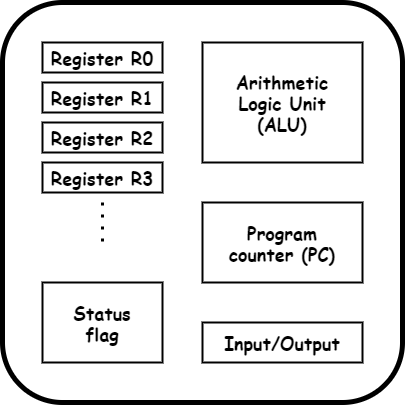
\includegraphics[scale = 0.5]{source/picture/Lab09/Processor_Image.png}
    \centering
\end{figure}

In which,
\begin{itemize}
	\item The \textbf{resistors} $R_0$, $R_1$, $R_2$, etc. are basically the CPU's internal RAM, and it will only have a small number of these. These resistors can either store numeric values or specific functions.
	\item The \textbf{arithmetic logic unit} is responsible for performing additions, subtractions, logic ands and ors, and other source of computation.
	\item The \textbf{status flags} registor is a collection of bits which will gives us information about the status of the CPU and the ALU.
	\item The \textbf{program counter} is used to store the address of where we are up to in our program. So, as the program is executed sequentially, the program counter increases. Furthermore, its value can be set depending on the result of something in the \textbf{status flags} register.
	\item \textbf{Input/Output} is how we are going to communicate, meaning getting the data in and out of the CPU.
\end{itemize}

\section{A Simple Processor}
The following figure shows a \textit{processor} that contains a number of nine-bit registers, a multiplexer, an adder/subtractor unit, and a control unit (finite state machine). Data is input to this system via the nine-bit DIN input. This data can be loaded through the nine-bit wide multiplexer into the various registers, such as $R_0$, . . . , $R_7$ and $A$. The multiplexer also allows data to be transferred from one register to another. The multiplexer’s output wires are called a bus in the figure because this term is often used for wiring that allows data to be transferred from one location in a system to another.\bigskip\\
Addition or subtraction of signed numbers is performed by using the multiplexer to first place one nine-bit number onto the bus wires and loading this number into register A. Once this is done, a second nine-bit number is placed onto the bus, the adder/subtractor unit performs the required operation, and the result is loaded into register G. The data in G can then be transferred to one of the other registers as required\\

\begin{figure}[h]
    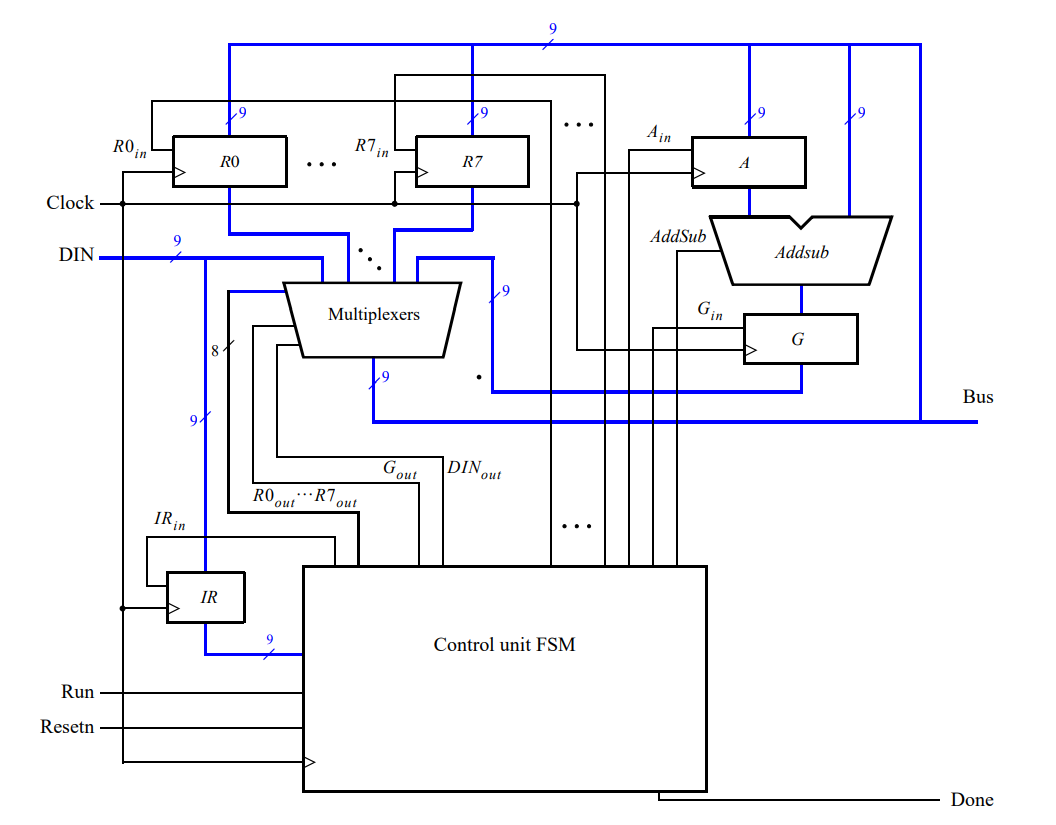
\includegraphics[scale = 0.75]{source/picture/Lab09/Simple_Processor_Figure.png}
    \centering
\end{figure}
\newpage

The system can perform different operations in each clock cycle, as governed by the control unit. This unit determines when particular data is placed onto the bus wires and it controls which of the registers is to be loaded with this data. For example, if the control unit asserts the signals $R0_{out}$ and $A_{in}$, then the multiplexer will place the contents of register $R_0$ onto the bus and this data will be loaded on the next active clock edge into $A$.\bigskip\\
The \textit{processor} executes operations specified in the form of \textit{instructions}. The following table lists the instructions the processor has to support. The left column shows the name of an instruction and its operands. The meaning of the syntax $Rx \xleftarrow{} [Ry]$ is that the contents of resister $Ry$ are loaded into register $Rx$. The \textbf{mv} (move) instruction allows data to be copied from one register to another. For the \textbf{mvi} (move immediate) instruction, the expression $Rx \xleftarrow{} D$ indicates that the nine-bit constant $D$ is loaded into register $Rx$.\\
\begin{table}[h]
    \begin{tabular}{l|l}
        Operation    & Function performed \\ \hline
        \textbf{mv} $Rx$,$Ry$   & $Rx \xleftarrow{} [Ry]$ \\ \hline
        \textbf{mvi} $Rx$,\#$D$ & $Rx \xleftarrow{} D$ \\ \hline
        \textbf{add} $Rx$,$Ry$  & $Rx\xleftarrow{}[Rx]+[Ry]$ \\ \hline
        \textbf{sub} $Ry$,$Ry$  & $Rx\xleftarrow{}[Rx]-[Ry]$
    \end{tabular}
    \centering
\end{table}

Each instruction can be encoded using the nine-bit format \textit{IIIXXXYYY} where \textit{III} specifies the instruction, \textit{XXX} gives the $Rx$ register, and \textit{YYY} gives the $Ry$ register. Although only two bits are needed to encode our four instructions, we are using three bits because other instructions will be added to the processor later. Assume that \textit{III} $=000$ for the \textbf{mv} instruction, 001 for \textbf{mvi}, 010 for \textbf{add}, and 011 for \textbf{sub}. Instructions are loaded from the the external input \textit{DIN}, and stored into the \textit{IR} register, using the connection indicated above. For the \textit{mvi} instruction, the \textit{YYY} field has no meaning, and the immediate data \#$D$ has to be supplied on the \textit{DIN} input in the clock cycle after the \textit{mvi} instruction word is stored into \textit{IR}.\bigskip\\
Some instructions, such as an addition or subtraction, take more than one clock cycle to complete, because multiple transfers have to be performed across the bus. The finite state machine in the control unit “steps through” such instructions, asserting the control signals needed in successive clock cycles until the instruction has completed. The processor starts executing the instruction on the \textit{DIN} input when the \textit{Run} signal is asserted and the processor asserts the \textit{Done} output when the instruction is finished. The following table indicates the control signals that can be asserted in each time step to implement the instructions in the previous table. Note that the only control signal asserted in time step 0 is \textit{IR}$_{in}$, so this time step is not shown in the table.\\
\begin{table}[h]
    \begin{tabular}{l|l|l|l}
     &\multicolumn{1}{c|}{T1}&\multicolumn{1}{c|}{T2}&\multicolumn{1}{c}{T3} \\ \hline
     (\textbf{mv}): $I_0$&$Ry_{out}$, $Rx_{in}$, \textit{done}&  &  \\ \hline
     (\textbf{mvi}): $I_1$&\textit{DIN}$_{out}$, $Rx_{in}$, \textit{done}&  &  \\ \hline
     (\textbf{add}): $I_2$&\textit{Rx}$_{out}$, $A_{in}$&\textit{Ry}$_{out}$, $G_{in}$&$G_{out}$, \textit{Rx}$_{in}$, \textit{done}\\ \hline
     (\textbf{sub}): $I_3$&\textit{Rx}$_{out}$, $A_{in}$&\textit{Ry}$_{out}$, $G_{in}$&$G_{out}$, \textit{Rx}$_{in}$, \textit{done} 
    \end{tabular}
    \centering
\end{table}
\newpage

The following block of \textbf{Verilog} code can be used to model the described processor.

\begin{lstlisting}[language=Verilog]
module pro(CLK,D_IN, RUN, RESET, DONE, BUS);
	input		[8:0]		D_IN;
	input					CLK, RESET, RUN;
	output	[8:0] 	BUS /*synthesis keep*/;
	output				DONE;
	
	wire		[8:0] 	reg0_out, reg1_out, reg2_out, reg3_out, reg4_out, reg5_out, reg6_out, reg7_out, regA_out, regG_out /*synthesis keep*/;
	wire		[8:0]		addsub_out /*synthesis keep*/;
	wire		[9:0]		reg_en /*synthesis keep*/;
	wire		[9:0]		multi_select /*synthesis keep*/;
	wire		[8:0] 	CODE /*synthesis keep*/;
	wire					MODE /*synthesis keep*/;
	
	regn	reg0 (.CLK(CLK), .EN(reg_en[0]), .IN(BUS), .OUT(reg0_out));
	regn	reg1 (.CLK(CLK), .EN(reg_en[1]), .IN(BUS), .OUT(reg1_out));
	regn	reg2 (.CLK(CLK), .EN(reg_en[2]), .IN(BUS), .OUT(reg2_out));
	regn	reg3 (.CLK(CLK), .EN(reg_en[3]), .IN(BUS), .OUT(reg3_out));
	regn	reg4 (.CLK(CLK), .EN(reg_en[4]), .IN(BUS), .OUT(reg4_out));
	regn	reg5 (.CLK(CLK), .EN(reg_en[5]), .IN(BUS), .OUT(reg5_out));
	regn	reg6 (.CLK(CLK), .EN(reg_en[6]), .IN(BUS), .OUT(reg6_out));
	regn	reg7 (.CLK(CLK), .EN(reg_en[7]), .IN(BUS), .OUT(reg7_out));
	regn	regA (.CLK(CLK), .EN(reg_en[8]), .IN(BUS), .OUT(regA_out));
	regn	regG (.CLK(CLK), .EN(reg_en[9]), .IN(addsub_out), .OUT(regG_out));
	regn	regI (.CLK(CLK), .EN(RUN), .IN(D_IN), .OUT(CODE));
	
	multiplexer inst0 (.IN0(reg0_out), .IN1(reg1_out), .IN2(reg2_out), .IN3(reg3_out), .IN4(reg4_out), 
							 .IN5(reg5_out), .IN6(reg6_out), .IN7(reg7_out), .IN8(regG_out), .IN9(D_IN), 
							 .SELECT(multi_select), .OUT(BUS));
							 
	addsub		inst1 (.MODE(MODE), .IN0(regA_out), .IN1(BUS), .OUT(addsub_out));
	
	control		inst2	(.CLK(CLK), .RUN(RUN), .RESET(RESET), .DONE(DONE), .CODE(CODE),
							 .REG_EN(reg_en), .MULTI_SELECT(multi_select), .MODE(MODE));
endmodule

module control(CLK, CODE, RUN, RESET, DONE, MODE, REG_EN, MULTI_SELECT);
	parameter MV=3'b000, MVI=3'b001, ADD=3'b010, SUB=3'b011, LDY=3'b100, UDX=3'b101, LDI=3'b110;  
	input		[8:0]		CODE;
	input					RUN, RESET, CLK;
	
	output	reg [9:0]	REG_EN;
	output	reg [9:0]	MULTI_SELECT;
	output	reg			DONE, MODE;
	
	reg		[2:0]		fsm_in, fsm_out /*synthesis keep */;

	
	//FSM
	always @(posedge CLK) begin
		fsm_out <= fsm_in;
	end
	
	always @(CODE) begin
		case (fsm_out)
			MV: fsm_in = CODE [8:6];
			MVI:fsm_in = LDI;
			ADD:fsm_in = LDY;
			SUB:fsm_in = LDY;
			LDY:fsm_in = UDX;
			UDX:fsm_in = CODE [8:6];
			default: fsm_in = CODE [8:6];
		endcase
	end
	
	//Control
	always @(fsm_in) begin
			if (fsm_in==MV) begin 
				MULTI_SELECT = {10{1'b0}} | (1<<CODE[2:0]);
				REG_EN 		 = {10{1'b0}} | (1<<CODE[5:3]);
				DONE			 = 1 ;
			end else 
			if (fsm_in==MVI) begin
				MULTI_SELECT = {10{1'b0}} | (1<<9);
				REG_EN 		 = {10{1'b0}} | (1<<CODE[5:3]);
				DONE			 = 0 ;
			end else
			if (fsm_in==LDI) begin
				REG_EN 		 = {10{1'b0}} | (0<<CODE[5:3]);
				DONE			 = 1 ;
			end else 
			if (fsm_in==ADD | fsm_in==SUB) begin
				MULTI_SELECT = {10{1'b0}} | (1<<CODE[5:3]);
				REG_EN 		 = {10{1'b0}} | (1<<8);
				DONE			 = 0 ;
			end else 
			if (fsm_in==LDY) begin
				MULTI_SELECT = {10{1'b0}} | (1<<CODE[2:0]);
				REG_EN 		 = {10{1'b0}} | (1<<9);
				DONE			 = 0 ;
			end else
			if (fsm_in==UDX) begin
				MULTI_SELECT = {10{1'b0}} | (1<<8);
				REG_EN 		 = {10{1'b0}} | (1<<CODE[5:3]);
				DONE			 = 1 ; 
			end
			
			if (fsm_in==ADD) MODE = 1'b0 ;
			if (fsm_out==SUB)MODE = 1'b1 ;
			
		end

endmodule

module multiplexer(IN0, IN1, IN2, IN3, IN4, IN5, IN6, IN7, IN8, IN9, SELECT, OUT);
	input		[8:0] 	IN0, IN1, IN2, IN3, IN4, IN5, IN6, IN7, IN8, IN9;
	input		[9:0]		SELECT;
	output	[8:0]		OUT /*synthesis keep*/;
	
	assign	OUT = IN0 & {9{SELECT[0]}} |
						IN1 & {9{SELECT[1]}} |
						IN2 & {9{SELECT[2]}} |
						IN3 & {9{SELECT[3]}} |
						IN4 & {9{SELECT[4]}} |
						IN5 & {9{SELECT[5]}} |
						IN6 & {9{SELECT[6]}} |
						IN7 & {9{SELECT[7]}} |
						IN8 & {9{SELECT[8]}} |
						IN9 & {9{SELECT[9]}} ;
endmodule

module addsub(MODE, IN0, IN1, OUT);
	parameter ADD=1'b0, SUB=1'b1;
	
	input		[8:0]	IN0, IN1 /*synthesis keep*/;
	input				MODE;
	output 	reg[8:0]	OUT;
	
	
	always @(IN0, IN1) begin
		if (MODE==ADD) OUT = IN1 + IN0;
		else OUT = IN1 - IN0;
	end
	
	
endmodule

module regn(IN, EN, CLK, OUT);
parameter n = 9;
	input 	[n-1:0] IN;
	input 	EN, CLK;
	output 	reg [n-1:0] OUT;
		
	always @(posedge CLK)
		if (EN)
			OUT <= IN;
endmodule
\end{lstlisting}

Using \textbf{Quartus}, we can generate a schematic block diagram and a waveform simulation, and the results are as followed.

\begin{figure}[h]
    \centering
    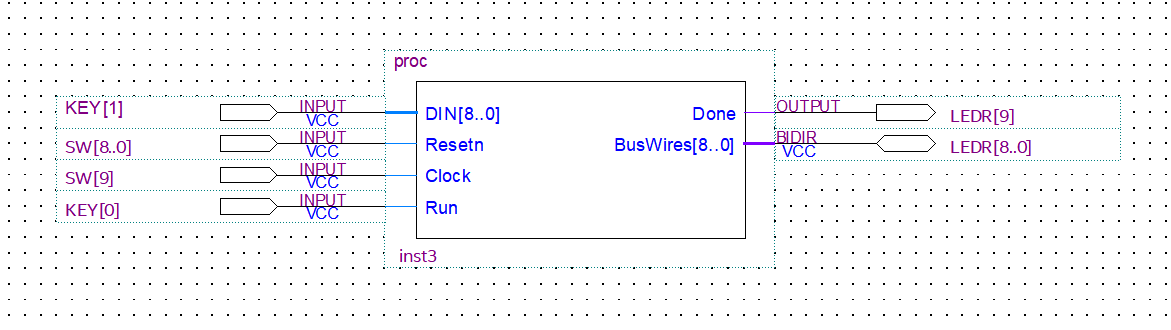
\includegraphics[scale = 0.5]{source/picture/Lab09/Lab9_1.png}
\end{figure}
\clearpage
\begin{figure}[h]
    \centering
    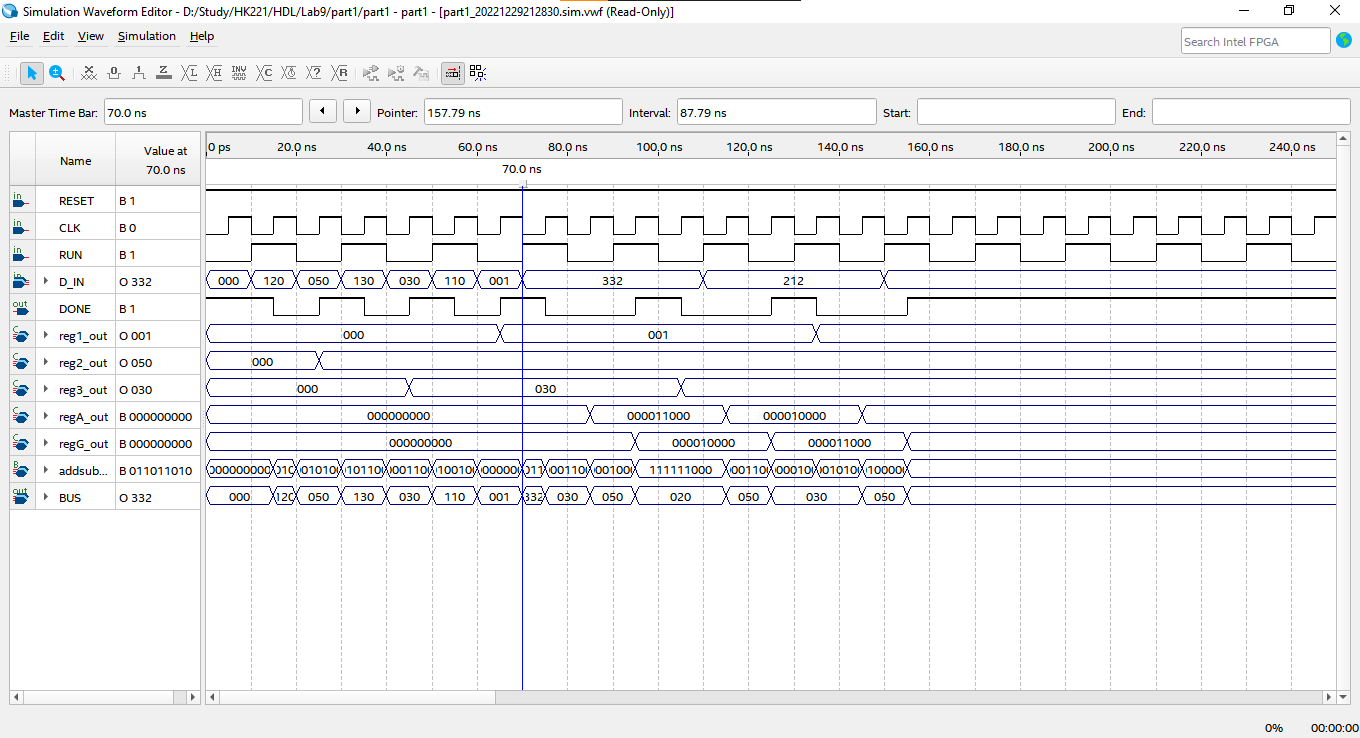
\includegraphics[width = \textwidth]{source/picture/Lab09/Lab9_1_stimulation.png}
\end{figure}

Here are some explanations for the simulation result above:
\begin{itemize}
    \item At $t=10ns$, the instruction 120 (9'b001010000) $\iff$ "\textbf{mvi} R2" is loaded into processor via \textbf{Run} signal, then at $t=15ns$ it is executed \textbf{Run} signal. In the next clock pulse (at $t=25ns$), the \textbf{value 050 is loaded into R2} and the signal \textbf{Done} is immediately returned. \textbf{This operation takes 2 clock pulses to complete.}
    \item At $t=20ns$, the instruction 120 (9'b001011000) $\iff$ "\textbf{mvi} R3" is loaded into processor via \textbf{Run} signal, then at $t=25ns$ it is executed. In the next clock pulse (at $t=35ns$), the \textbf{value 050 is loaded into R2} and the signal \textbf{Done} is immediately returned. \textbf{This operation takes 2 clock pulses to complete.}
    \item At $t=50ns$, the instruction 110 (9'b001001000) $\iff$ "\textbf{mvi} R1" is loaded into BUS\_WIRE, then at $t=55ns$ flows to the processor via the \textbf{Run} signal. In the next clock pulse (at $t=65ns$), the \textbf{value 001 is loaded into R1} and the signal \textbf{Done} is immediately returned. \textbf{This operation takes 2 clock pulses to complete.}
    \item At $t=70ns$, the instruction 332 (9'b011011010) $\iff$ "\textbf{sub} R3,R2" is loaded into processor via \textbf{Run} signal, then it is executed at $t=75ns$ - this is the reason why at this time, the BUS\_WIRE hold the value of R3 (020), immediately, this value flows to the \textbf{Addsub} module. At the next clock pulse, the value of the $R_2$ (050) is loaded into the BUS\_WIRE, then flow to {Addsub} to compute the value, in this case, this module minus 020 from 050 and save into $R_3$. This operation takes 3 clock pulses to complete.
\end{itemize}
\clearpage
Let's take this one step further by adding a memory module and a counter to our processor. The counter is used to read the contents of successive addresses in the memory, and this data is provided to the processor as a stream of instructions. To simplify the design and testing of this circuit we will use separate clock signals, PClock and MClock, for the processor and the memory.

\begin{figure}[h]
    \centering
    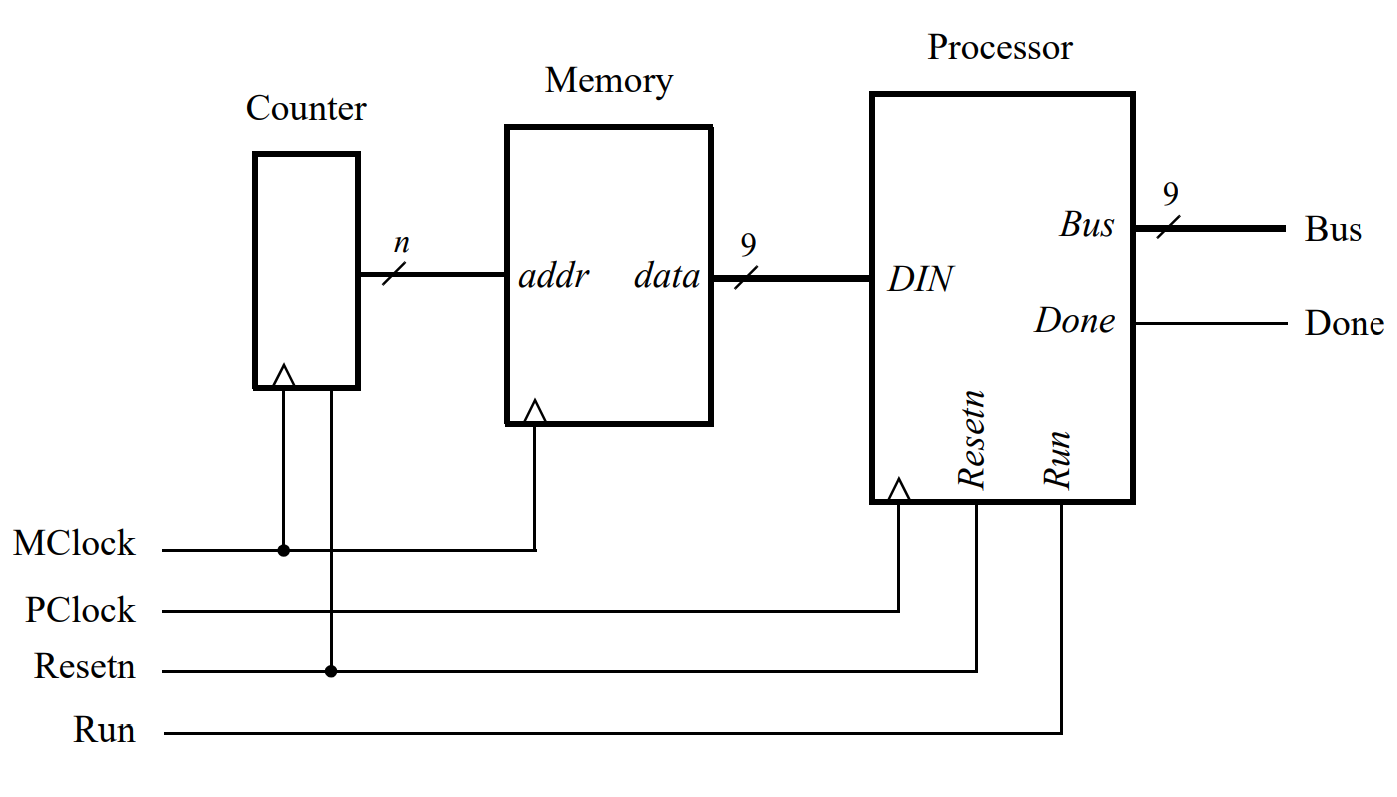
\includegraphics[width=5.5in]{source/picture/Lab09/Simple_Processor_W_Counter.png}
\end{figure}

The counter we will be using is just a simple mod-32 counter. The \textbf{verilog} code for the counter is as followed.

\begin{lstlisting}[language=Verilog]
module counterv(CLK,RESET,Q);
	input CLK,RESET;
	output reg [4:0] Q;
	
	
	always@(posedge CLK) begin
		if(!RESET) Q<=0;
		else Q<=Q+1;
	end
	
endmodule
\end{lstlisting}

Next, the memory we will be using will be called a \textit{synchronous read-only memory (synchronous ROM)} since it has only a read port and no write port. Using the Quartus IP Catalog tool, we can create this memory module as follow.

\begin{figure}[h]
    \centering
    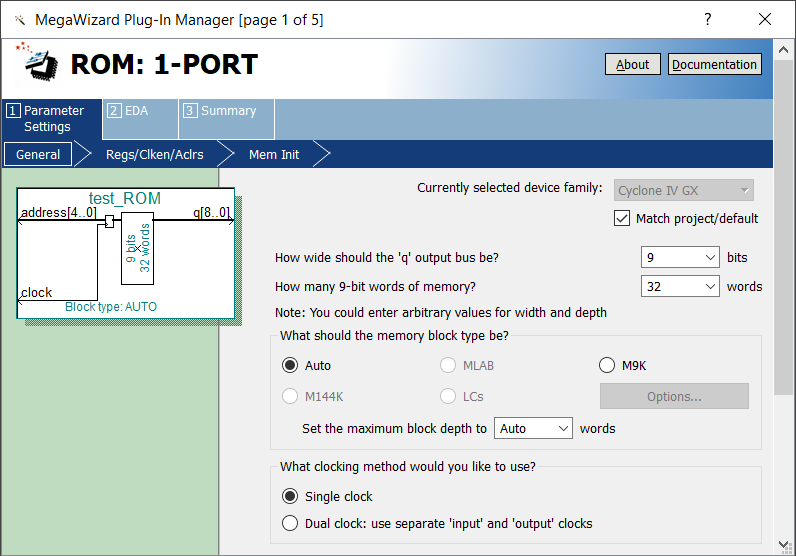
\includegraphics[width = 5.5in]{source/picture/Lab09/Create_ROM_1.png}
\end{figure}

\begin{figure}[h]
    \centering
    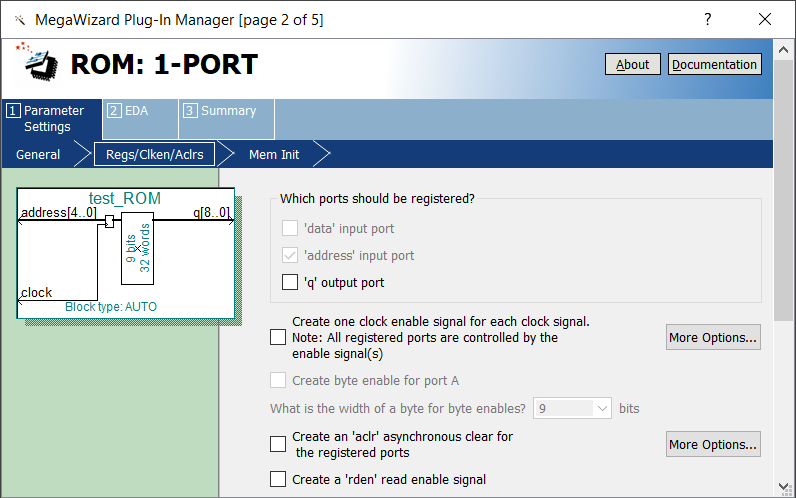
\includegraphics[width = 5.5in]{source/picture/Lab09/Create_ROM_2.png}
\end{figure}

We can initialize the initial content of the memory by using a \textit{Memory Initialization File} [.mif]. So we created such file, named \textit{inst\_mem.mif} and its content is as followed.
\newpage

\begin{lstlisting}[language=verilog]

WIDTH=9;
DEPTH=32;

ADDRESS_RADIX=UNS;
DATA_RADIX=OCT;

CONTENT BEGIN
    0   :   100;
    1   :   005;
    2   :   010;
    3   :   201;
    4   :   300;
    [5..31]  :   000;
END;
\end{lstlisting}

\newpage

Using \textbf{Quartus}, we can generate a schematic block diagram and a waveform simulation. The results are as followed. (Click \href{https://drive.google.com/file/d/1bG-vFAlYrJjy5utJ4DoETYb3e9kJMEU5/view?usp=sharing}{here} for a more detailed schematic and \href{https://drive.google.com/file/d/1yXu4M1fxIND9-f9YMr3JbLg8KXuOInd-/view?usp=sharing}{here} for a more detailed simulation result)

\begin{figure}[h]
    \centering
    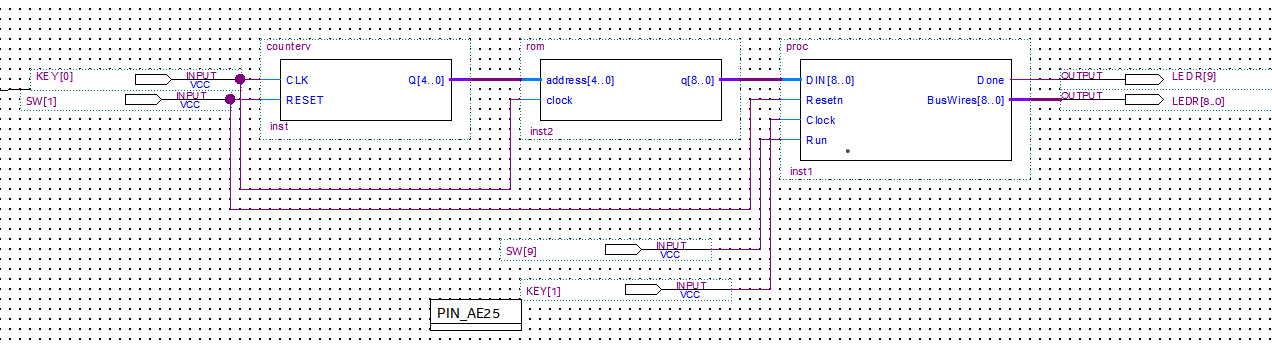
\includegraphics[width=6.1in]{source/picture/Lab09/Lab9_2.png}
\end{figure}

\begin{figure}[h]
    \centering
    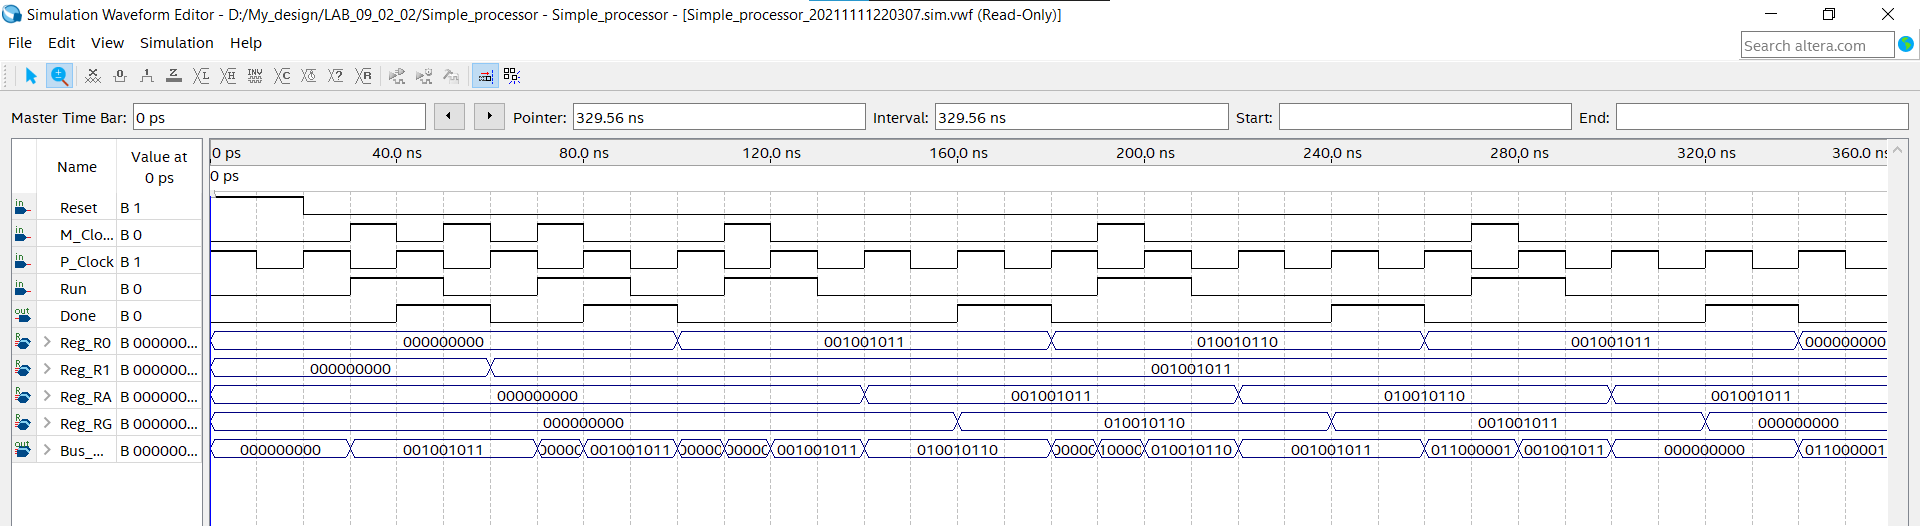
\includegraphics[width=6.1in]{source/picture/Lab09/Simple_Processor_W_Counter_Simulation.png}
\end{figure}

Here are some explanations for the simulation result above:
\begin{itemize}
    \item The instructions and instruction order are exactly the same as with the previous simulation result. The interesting thing here is the way that we load the instruction to our processor. Therefore, we will focus more on that aspect.
    \item At $t=30ns$, there is an \textbf{M\_Clock} signal to start both the counter and the ROM. After this, we are at the address 00 : 001001011. Then there's a \textbf{Run} signal and the processor loads the instruction 001001011 in.
    \item At $t=50ns$, another \textbf{M\_Clock} signal moves us to the next address 01 : 001001011. The processor then proceeds to load the value 001001011 into the $R_1$ register.
    \item At $t=70ns$, another \textbf{M\_Clock} signal moves us to the next address 02 : 000000001. The processor then proceeds to load the value of register $R_1$ into register $R_0$.
    \item At $t=110ns$, another \textbf{M\_Clock} signal moves us to the next address 03 : 010000001. The processor then proceeds to add the value of registers $R_1$ and $R_0$ together, then registers that value into $R_0$.
    \item At $t=190ns$, another \textbf{M\_Clock} signal moves us to the next address 04 : 011000001. The processor then proceeds to subtracts the value of registers $R_1$ from $R_0$, then registers that value into $R_0$.
    \item At $t=270ns$, another \textbf{M\_Clock} signal moves us to the next address 05 : 011000001. The processor then proceeds to subtracts the value of registers $R_1$ from $R_0$, then registers that value into $R_0$.
\end{itemize}